\documentclass{article}\usepackage[]{graphicx}\usepackage[]{xcolor}
% maxwidth is the original width if it is less than linewidth
% otherwise use linewidth (to make sure the graphics do not exceed the margin)
\makeatletter
\def\maxwidth{ %
  \ifdim\Gin@nat@width>\linewidth
    \linewidth
  \else
    \Gin@nat@width
  \fi
}
\makeatother

\definecolor{fgcolor}{rgb}{0.345, 0.345, 0.345}
\newcommand{\hlnum}[1]{\textcolor[rgb]{0.686,0.059,0.569}{#1}}%
\newcommand{\hlstr}[1]{\textcolor[rgb]{0.192,0.494,0.8}{#1}}%
\newcommand{\hlcom}[1]{\textcolor[rgb]{0.678,0.584,0.686}{\textit{#1}}}%
\newcommand{\hlopt}[1]{\textcolor[rgb]{0,0,0}{#1}}%
\newcommand{\hlstd}[1]{\textcolor[rgb]{0.345,0.345,0.345}{#1}}%
\newcommand{\hlkwa}[1]{\textcolor[rgb]{0.161,0.373,0.58}{\textbf{#1}}}%
\newcommand{\hlkwb}[1]{\textcolor[rgb]{0.69,0.353,0.396}{#1}}%
\newcommand{\hlkwc}[1]{\textcolor[rgb]{0.333,0.667,0.333}{#1}}%
\newcommand{\hlkwd}[1]{\textcolor[rgb]{0.737,0.353,0.396}{\textbf{#1}}}%
\let\hlipl\hlkwb

\usepackage{framed}
\makeatletter
\newenvironment{kframe}{%
 \def\at@end@of@kframe{}%
 \ifinner\ifhmode%
  \def\at@end@of@kframe{\end{minipage}}%
  \begin{minipage}{\columnwidth}%
 \fi\fi%
 \def\FrameCommand##1{\hskip\@totalleftmargin \hskip-\fboxsep
 \colorbox{shadecolor}{##1}\hskip-\fboxsep
     % There is no \\@totalrightmargin, so:
     \hskip-\linewidth \hskip-\@totalleftmargin \hskip\columnwidth}%
 \MakeFramed {\advance\hsize-\width
   \@totalleftmargin\z@ \linewidth\hsize
   \@setminipage}}%
 {\par\unskip\endMakeFramed%
 \at@end@of@kframe}
\makeatother

\definecolor{shadecolor}{rgb}{.97, .97, .97}
\definecolor{messagecolor}{rgb}{0, 0, 0}
\definecolor{warningcolor}{rgb}{1, 0, 1}
\definecolor{errorcolor}{rgb}{1, 0, 0}
\newenvironment{knitrout}{}{} % an empty environment to be redefined in TeX

\usepackage{alltt}
\usepackage[T1]{fontenc}
\IfFileExists{upquote.sty}{\usepackage{upquote}}{}
\begin{document}

This is an example LaTeX document with some embedded R code woven in for convenience.

\begin{knitrout}
\definecolor{shadecolor}{rgb}{0.969, 0.969, 0.969}\color{fgcolor}\begin{kframe}
\begin{alltt}
\hlstd{x} \hlkwb{=} \hlnum{1}\hlopt{:}\hlnum{10}
\hlstd{y}  \hlkwb{=} \hlstd{x} \hlopt{^} \hlnum{2}
\hlkwd{plot}\hlstd{(x, y,} \hlkwc{main} \hlstd{=} \hlstr{"This is a graph"}\hlstd{)}
\end{alltt}
\end{kframe}
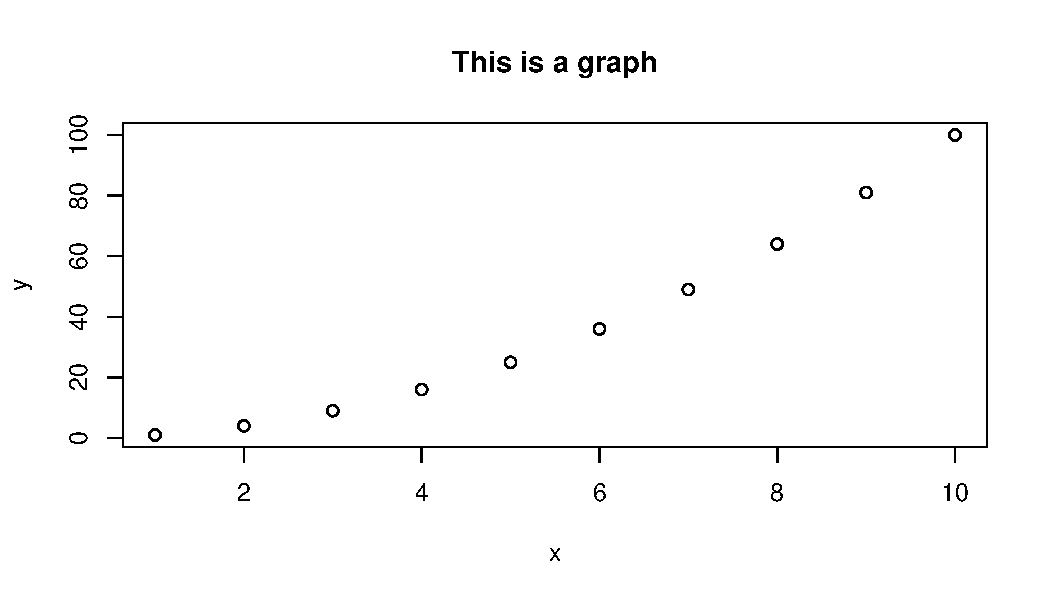
\includegraphics[width=\maxwidth]{figure/foo-1} 
\end{knitrout}

Inline expressions can be written by using the
\verb|\Sexpr{}| convention, e.g. $\pi=3.1415927$
and \ensuremath{2.3492\times 10^{7}} and 0.5, 1, 1.5, 2, 2.5, 3, 3.5, 4, 4.5, 5.

\subsection*{A different subsection}
We can insert graphs without displaying the code.
This can be done using the \texttt{echo = FALSE}
command within the code chunk argument list.

\begin{knitrout}
\definecolor{shadecolor}{rgb}{0.969, 0.969, 0.969}\color{fgcolor}
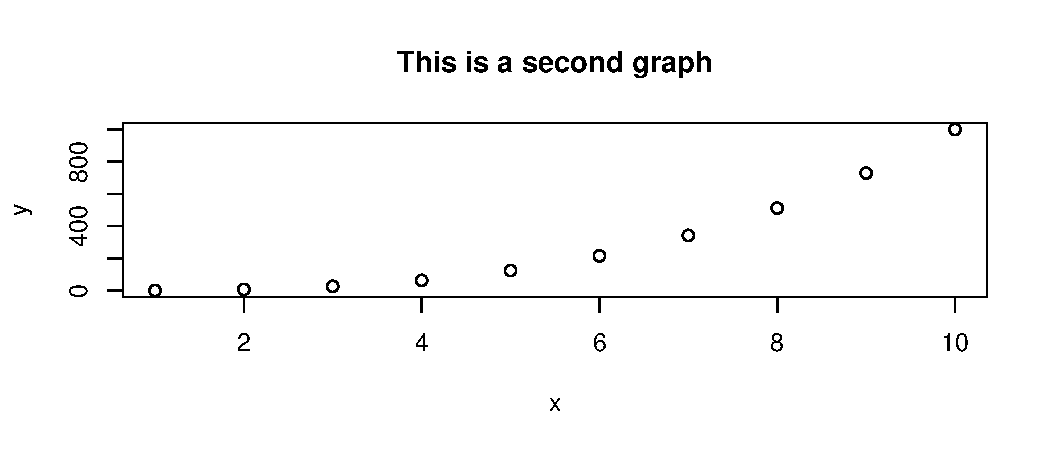
\includegraphics[width=\maxwidth]{figure/foo2-1} 
\end{knitrout}

Any R code can be run within the code chunks
provided by knitr. This next example loads up
\texttt{ggplot2}, and the code creates a nice looking
density histogram.

\begin{knitrout}
\definecolor{shadecolor}{rgb}{0.969, 0.969, 0.969}\color{fgcolor}\begin{kframe}
\begin{alltt}
\hlkwd{require}\hlstd{(ggplot2)}
\end{alltt}


{\ttfamily\noindent\itshape\color{messagecolor}{\#\# Loading required package: ggplot2}}\begin{alltt}
\hlstd{my_data} \hlkwb{=} \hlkwd{data.frame}\hlstd{(}\hlkwc{returns} \hlstd{=} \hlkwd{c}\hlstd{(}\hlnum{0.03}\hlstd{,} \hlnum{0.04}\hlstd{,} \hlnum{0.05}\hlstd{,}
\hlnum{0.032}\hlstd{,} \hlnum{0.01}\hlstd{,} \hlnum{0.23}\hlstd{,} \hlnum{0.4}\hlstd{,} \hlnum{0.05}\hlstd{,} \hlnum{0.066}\hlstd{,} \hlnum{0.5}\hlstd{),}
\hlkwc{stock} \hlstd{=} \hlkwd{c}\hlstd{(}\hlstr{"SPY"}\hlstd{,} \hlstr{"CVX"}\hlstd{,} \hlstr{"SPY"}\hlstd{,} \hlstr{"SPY"}\hlstd{,} \hlstr{"XOM"}\hlstd{))}

\hlkwd{ggplot}\hlstd{(my_data,} \hlkwd{aes}\hlstd{(}\hlkwc{x} \hlstd{= returns,} \hlkwc{fill} \hlstd{= stock))} \hlopt{+}
\hlkwd{geom_density}\hlstd{(}\hlkwc{alpha} \hlstd{=} \hlnum{0.2}\hlstd{)}
\end{alltt}
\end{kframe}
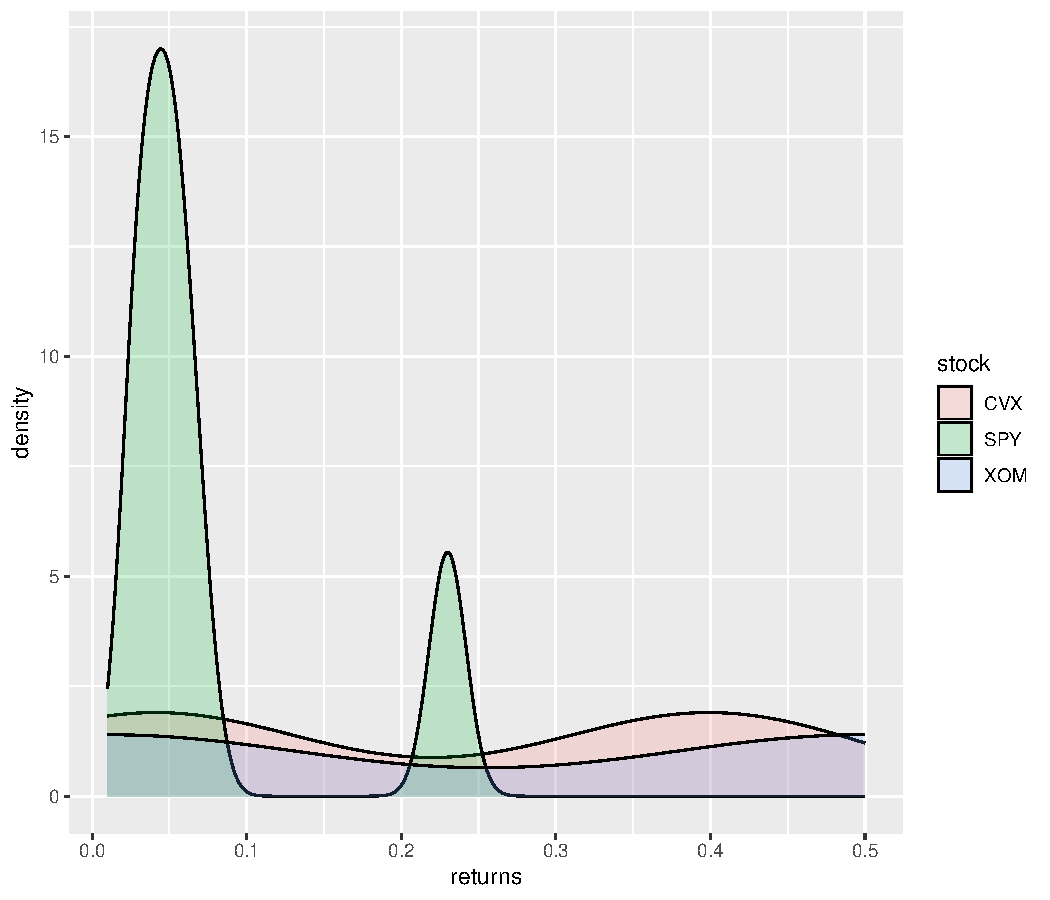
\includegraphics[width=\maxwidth]{figure/foo3-1} 
\end{knitrout}

\end{document}
